\documentclass[12pt]{article}
\usepackage{amsthm,amssymb,amsfonts,amsmath,amstext,systeme}
\usepackage{graphicx,float}
\usepackage{tabularx}

\marginparwidth 0pt
\oddsidemargin -1.2 truecm
\evensidemargin  0pt 
\marginparsep 0pt
\topmargin -2.2truecm
\linespread{1}
\textheight 25.8 truecm
\textwidth 18.5 truecm
\newenvironment{remark}{\noindent{\bf Remark }}{\vspace{0mm}}
\newenvironment{remarks}{\noindent{\bf Remarks }}{\vspace{0mm}}
\newenvironment{question}{\noindent{\bf Question }}{\vspace{0mm}}
\newenvironment{questions}{\noindent{\bf Questions }}{\vspace{0mm}}
\newenvironment{note}{\noindent{\bf Note }}{\vspace{0mm}}
\newenvironment{summary}{\noindent{\bf Summary }}{\vspace{0mm}}
\newenvironment{back}{\noindent{\bf Background}}{\vspace{0mm}}
\newenvironment{conclude}{\noindent{\bf Conclusion}}{\vspace{0mm}}
\newenvironment{concludes}{\noindent{\bf Conclusions}}{\vspace{0mm}}
\newenvironment{dill}{\noindent{\bf Description of Dill's model}}{\vspace{0mm}}
\newenvironment{maths}{\noindent{\bf Mathematics needed}}{\vspace{0mm}}
\newenvironment{inst}{\noindent{\bf Instructions}}{\vspace{0mm}}
\newenvironment{notes}{\noindent{\bf Notes }}{\vspace{0mm}}
\newenvironment{theorem}{\noindent{\bf Theorem }}{\vspace{0mm}}
\newenvironment{example}{\noindent{\bf Example }}{\vspace{0mm}}
\newenvironment{examples}{\noindent{\bf Examples }}{\vspace{0mm}}
\newenvironment{topics}{\noindent{\bf Topics}}{\vspace{0mm}}
\newenvironment{outcomes}{\noindent{\bf Expected Learning Outcomes}}{\vspace{0mm}}
\newenvironment{lemma}{\noindent{\bf Lemma }}{\vspace{0mm}}
\newenvironment{solution}{\noindent{\it Solution}}{\vspace{2mm}}
\newcommand{\ds}{\displaystyle}
\newcommand{\un}{\underline}
\newcommand{\bs}{\boldsymbol}

\begin{document}

\baselineskip 18 pt
\begin{center}
	{\large \bf HKDSE MATH M2 Sample Paper}\\
	\vspace{2 mm}

\end{center}
\vspace{0.05cm}

\begin{enumerate}
	\item \textbf{HKDSE Math M2 Sample Paper Q1}\\
	Find $\displaystyle\frac{d}{dx}(\sqrt{2x})$ from first principles. \\(4 marks)


	\item \textbf{HKDSE Math M2 Sample Paper Q2}\\
	A snowball in a shape of sphere is melting with its volume decreasing at a constant rate of 4 cm$^3$s$^{-1}$. When its radius is 5 cm, find the rate of change of its radius. \\(4 marks)


	\item \textbf{HKDSE Math M2 Sample Paper Q3}\\
	The slope at any point $(x,y)$ of a curve is given by $\displaystyle\frac{dy}{dx} = 2x \ln{(x^2+1)}$. It is given that the curve passes through the point $(0,1)$.\\Find the equation of the curve. \\(4 marks)
		

	\item \textbf{HKDSE Math M2 Sample Paper Q4}\\
	Find $\displaystyle\int\left(x^2-\frac{1}{x}\right)^4 \,dx$. \\(4 marks)


	\item \textbf{HKDSE Math M2 Sample Paper Q5}\\
	By considering $\displaystyle\sin{\frac{\pi}{7}}\cos{\frac{\pi}{7}}\cos{\frac{2\pi}{7}}\cos{\frac{3\pi}{7}}$, find the value of $\displaystyle\cos{\frac{\pi}{7}}\cos{\frac{2\pi}{7}}\cos{\frac{3\pi}{7}}$. \\(4 marks)


	\item \textbf{HKDSE Math M2 Sample Paper Q6}\\
	Let $C$ be the curve $3e^{x-y} = x^2+y^2+1$. \\
	Find the equation of the tangent to $C$ at the point $(1,1)$. \\(5 marks)


	\item \textbf{HKDSE Math M2 Sample Paper Q7}\\
	Solve the system of linear equations
	$$\left\{\begin{matrix}
		x & + & 7y & - & 6z & = & -4\\
		3x & - & 4y & + & 7z & = & 13\\
		4x & + & 3y & + & z & = & 9\\
	\end{matrix}\right..$$ \\(5 marks)

	\item\textbf{HKDSE Math M2 Sample Paper Q8}
	\begin{enumerate}
		\item [(a)]Using integration by parts, find $\displaystyle\int x\cos{x}\,dx$. 
		\item [(b)]The \textbf{inner surface} of a container is formed by revolving the curve $y = -\cos{x}$ (for $0 \leq x \leq \pi$) about the $y$-axis (see Figure 1). Find the capacity of the container. 
		\begin{figure}[H]
			\centering
			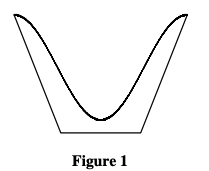
\includegraphics[width = .5\linewidth]{SPFigure1}
		\end{figure}
	\end{enumerate}
	(6 marks)


	\item \textbf{HKDSE Math M2 Sample Paper Q9}\\
	Let $\overrightarrow{OA} = 4\textbf{i} +3 \textbf{j}$, $\overrightarrow{OB} = 3 \textbf{j} +\textbf {k}$ and $\overrightarrow{OC} = 3\textbf{i} + \textbf{j} +5\textbf {k}$. Figure 2 shows the parallelepiped $OADBECFG$ formed by $\overrightarrow{OA}$, $\overrightarrow{OB}$ and $\overrightarrow{OC}$. 
	\begin{figure}[H]
		\centering
		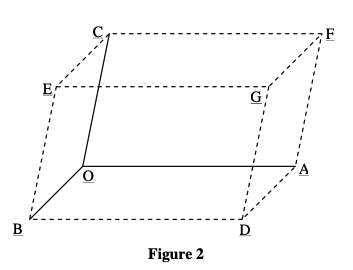
\includegraphics[width = .5\linewidth]{SPFigure2}
	\end{figure}
	\begin{enumerate}
		\item [(a)]Find the area of the parallelogram $OADB$.  
		\item [(b)]Find the volume of the parallelepiped $OADBECFG$.
		\item [(c)]If $C'$ is a point different from $C$ such that the volume of the parallelepiped formed by $\overrightarrow{OA}$, $\overrightarrow{OB}$ and $\overrightarrow{OC'}$ is the same as that of $OADBECFG$, find a possible vector of $\overrightarrow{OC'}$.
	\end{enumerate}
	(6 marks)

	\item \textbf{HKDSE Math M2 Sample Paper Q10}\\
	Let $0^{\circ} < \theta < 180^{\circ}$ and define $A = \begin{pmatrix}\cos{\theta}&-\sin{\theta}\\\sin{\theta}&\cos{\theta}\\\end{pmatrix}$. 
	\begin{enumerate}
		\item [(a)]Prove, by mathematical induction, that \\
		$A^n = \begin{pmatrix}\cos{n\theta}&-\sin{n\theta}\\\sin{n\theta}&\cos{n\theta}\\\end{pmatrix}$\\
		for all positive integers $n$.
		\item [(b)]Solve $\sin{3\theta} + \sin{2\theta} + \sin{\theta} = 0$.
		\item [(c)]It is given that $A^3 + A^2 + A = \begin{pmatrix}a&0\\0&a\\\end{pmatrix}$.\\Find the value(s) of $a$. 
	\end{enumerate}
	(8 marks)

	\item \textbf{HKDSE Math M2 Sample Paper Q11}\\
	Let $A = \begin{pmatrix}
		2 & 0 & 0\\
		1 & 1 & 0\\
		1 & 0 & 1\\
	\end{pmatrix}$, $P = \begin{pmatrix}
		0 & 0 & 1\\
		0 & 1 & 1\\
		1 & 1 & 1\\
	\end{pmatrix}$ and $P = \begin{pmatrix}
		1 & 0 & 0\\
		0 & 1 & 0\\
		0 & 0 & 2\\
	\end{pmatrix}$.
	\begin{enumerate}
		\item [(a)]Let $I$ and $O$ be the $3\times3$ identity matrix and zero matrix respectively. 
		\begin{enumerate}
			\item [(i)]Prove that $P^3 -2P^2 - P + I = O$.
			\item [(ii)]Using the result of (i), or otherwise, find $P^{-1}$.
		\end{enumerate}
		(5 marks)
		\item [(b)]
		\begin{enumerate}
			\item [(i)]Prove that $D = P^{-1}AP$. 
			\item [(ii)]Prove that $D$ and $A$ are non-singular. 
			\item [(iii)]Find $(D^{-1})^{100}$. \\
			Hence, or otherwise, find $(A^{-1})^{100}$.
		\end{enumerate}
		(7 marks)
	\end{enumerate}


	\item \textbf{HKDSE Math M2 Sample Paper Q12}\\
	Let $\displaystyle f(x) = \frac{4}{x-1} - \frac{4}{x+1} -1$, where $x \neq \pm 1$.
	\begin{enumerate}
		\item [(a)]
		\begin{enumerate}
			\item [(i)]Find the $x$- and $y$-intercept(s) of the graph of $y = f(x)$. 
			\item [(ii)]Find $f'(x)$ and prove that 
			$$f''(x) = \displaystyle\frac{16(3x^2 + 1)}{(x-1)^3(x+1)^3}$$
			for $x \neq \pm 1$. 
			\item [(iii)]For the graph of $y = f(x)$, find all the extreme points and show that there are no points of inflexion.
		\end{enumerate}
		(6 marks)
		\item [(b)]Find all the asymptote(s) of the graph of $y = f(x)$. \\(2 marks)
		\item [(c)]Sketch the graph of $y = f(x)$. \\(3 marks)
		\item [(d)]Let $S$ be the area bounded by the graph of $y = f(x)$, the straight lines $x = 3$, $x = a $ $(a > 3)$ and $y = -1$. \\
		Find $S$ in terms of $a$. \\
		Deduce that $S < 4\ln{2}$. \\(3 marks)
  	\end{enumerate}

	\item \textbf{HKDSE Math M2 Sample Paper Q13}
	\begin{enumerate}
		\item[(a)]Let $a > 0$ and $f(x)$ be a continuous function. \\
		Prove that $\displaystyle\int_{0}^a f(x) \,dx = \int_{0}^a f(a-x) \,dx$.\\
		Hence, prove that $\displaystyle\int_{0}^a f(x) \,dx = \frac{1}{2}\int_{0}^a [f(x) + f(a-x)] \,dx$. \\(3 marks)
		\item[(b)]Show that $\displaystyle\int_0^1 \frac{dx}{x^2-x+1} = \frac{2\sqrt{3}\pi}{9}$. \\(5 marks)
		\item[(c)]Using (a) and (b), or otherwise, evaluate $\displaystyle\int _0^1 \frac{dx}{(x^2-x+1)(e^{2x-1}+1)}$. \\(6 marks)
	\end{enumerate}


	\item \textbf{HKDSE Math M2 Sample Paper Q14}\\
	In Figure 3, $\triangle ABC$ is an acute-angled triangle, where $O$ and $H$ are the circumcentre and orthocentre respectively. Let $\overrightarrow{OA} = \textbf{a}$, $\overrightarrow{OB} = \textbf{b}$, $\overrightarrow{OC} = \textbf{c}$ and $\overrightarrow{OH} = \textbf{h}$.
	\begin{figure}[H]
		\centering
		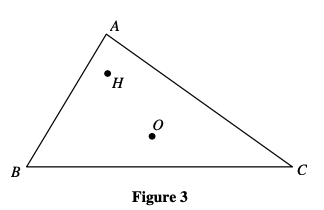
\includegraphics[width = .5\linewidth]{SPFigure3}
	\end{figure}
	\begin{enumerate}
		\item [(a)]Show that $(\textbf{h} - \textbf{a})//(\textbf{b}+\textbf{c})$. \\(3 marks)
		\item [(b)]Let $\textbf{h} - \textbf{a} = t(\textbf{b}+\textbf{c})$, where $t$ is a non-zero constant.\\
		Show that 
		\begin{enumerate}
			\item [(i)]$t(\textbf{b}+\textbf{c}) + \textbf{a} - \textbf{b} = s(\textbf{c}+\textbf{a})$ for some scalar $s$, 
			\item [(ii)]$(t-1)(\textbf{b}-\textbf{a})\cdot (\textbf{c}-\textbf{a}) = 0$.
		\end{enumerate}
		(5 marks)
		\item[(c)]Express $\textbf{h}$ in terms of $\textbf{a}$, $\textbf{b}$ and $\textbf{c}$. \\(2 marks)
	\end{enumerate}
\end{enumerate}
\end{document}